% !TeX encoding = UTF-8
% !TeX program = xelatex
% !TeX spellcheck = en_US

\documentclass[degree=doctor]{bnuthesis}
  % 学位 degree:
  %   doctor | master | bachelor | postdoc
  % 学位类型 degree-type:
  %   academic（默认）| professional
  % 语言 language
  %   chinese（默认）| english
  % 字体库 fontset
  %   windows | mac | fandol | ubuntu
  % 2026 年编写规则要求中文宋体、标题黑体，英文 Times New Roman。
  % 终稿应核对实际字体及培养单位的补充要求。


% 论文基本配置，加载宏包等全局配置
% !TeX root = ./bnuthesis-example.tex

% 论文基本信息配置

\bnusetup{
  %******************************
  % 注意：
  %   1. 配置里面不要出现空行
  %   2. 不需要的配置信息可以删除
  %   3. 建议先阅读文档中所有关于选项的说明
  %******************************
  %
  % 输出格式
  %   选择打印版（print）或用于提交的电子版（electronic）。
  %   正文每章另起页；2026 年规则未要求每章必须从奇数页开始。
  %
  output = print,
  %
  % 标题
  %   可使用“\\”命令手动控制换行
  %
  title  = {北京师范大学学位论文 \LaTeX{} 模板使用示例文档 v\version},
  title* = {AN INTRODUCTION TO \LaTeX{} THESIS TEMPLATE OF BEIJING NORMAL UNIVERSITY v\version},
  %
  % 学位
  %   1. 学术型
  %      - 中文
  %        需注明所属的学科门类，例如：
  %        哲学、经济学、法学、教育学、文学、历史学、理学、工学、农学、医学、
  %        军事学、管理学、艺术学
  %      - 英文
  %        博士：Doctor of Philosophy
  %        硕士：
  %          哲学、文学、历史学、法学、教育学、艺术学门类，公共管理学科
  %          填写“Master of Arts“，其它填写“Master of Science”
  %   2. 专业型
  %      直接填写专业学位的名称，例如：
  %      教育博士、工程硕士等
  %      Doctor of Education, Master of Engineering
  %
  degree-name  = {理学博士},
  degree-name* = {Doctor of Science},
  %
  % 培养单位
  %   填写所属院系的全名
  %
  department = {数学科学学院},
  %
  % 学科
  %   1. 学术型学位
  %      获得一级学科授权的学科填写一级学科名称，其他填写二级学科名称
  %   2. 工程硕士
  %      工程领域名称
  %   3. 其他专业型学位
  %      不填写此项
  %
  discipline  = {计算数学},
  discipline* = {Mathematics and Applied Mathematics (Liyun)},
  %
  % 学号
  %
  student-id  = {202431130057},
  %
  % 姓名
  %
  author  = {阙嘉豪},
  author* = {Que Jiahao},
  %
  % 指导教师
  %   中文姓名和职称之间以英文逗号“,”分开，下同
  %
  supervisor  = {陈华杰, 教授},
  supervisor* = {Professor Chen Huajie},
  supervisor-department = {数学科学学院},
  %
  % 副指导教师
  %
  associate-supervisor  = {陈华杰, 教授},
  associate-supervisor* = {Professor Chen Huajie},
  %
  % 联合指导教师
  %
  % co-supervisor  = {某某某, 教授},
  % co-supervisor* = {Professor Mou Moumou},
  %
  % 日期
  %   使用 ISO 格式；默认为当前时间
  %
  % date = {2019-07-07},
  %
  % 是否在中文封面后的空白页生成书脊（默认 false）
  %
  include-spine = true,
  %
  % 密级和年限
  %   秘密, 机密, 绝密
  %
  % secret-level = {秘密},
  % secret-year  = {10},
  %
  % 博士后专有部分
  %
  % clc                = {分类号},
  % udc                = {UDC},
  % id                 = {编号},
  % discipline-level-1 = {计算机科学与技术},  % 流动站（一级学科）名称
  % discipline-level-2 = {系统结构},          % 专业（二级学科）名称
  % start-date         = {2011-07-01},        % 研究工作起始时间
}

% 载入所需的宏包

% 定理类环境宏包
\usepackage{amsthm}
% 也可以使用 ntheorem
% \usepackage[amsmath,thmmarks,hyperref]{ntheorem}

\bnusetup{
  % 西文使用 Times New Roman、Arial 和 Courier New；中文使用 Windows 中易字体
  font = times,
  cjk-font = windows,
  % 数学字体
  math-style = TeX,  % GB | ISO | TeX
  less-than-or-equal = slanted,
  math-font  = newcm,  % sitx | xits | libertinus | newcm
}

% 可以使用 nomencl 生成符号和缩略语说明
% \usepackage{nomencl}
% \makenomenclature

% 表格加脚注
\usepackage{threeparttable}

% 表格中支持跨行
\usepackage{multirow}

% 固定宽度的表格。
% \usepackage{tabularx}

% 跨页表格
\usepackage{longtable}

% 量和单位
\usepackage{siunitx}

% 参考文献使用 BibTeX + natbib 宏包
% 顺序编码制
% \usepackage[sort]{natbib}
% \bibliographystyle{bnuthesis-numeric}

% 本例按已确认的例外保留：文献表按著者-出版年排序，正文用数字上标。
% 该组合不属于规则列出的两种标准配套方案，正式提交前应向培养单位确认。
% 中文著者排序依赖 .bib 条目中的拼音 key 字段，新增条目时应核对。
% 正文演示不切换引文制度；其他配套方案见 data/chap04.tex 的代码说明。
\usepackage{natbib}
\bibliographystyle{bnuthesis-author-year-bnu}

% 著者-出版年制
% \usepackage{natbib}
% \bibliographystyle{bnuthesis-author-year}

% 参考文献使用 BibLaTeX 宏包
% \usepackage[backend=biber,style=bnuthesis-numeric]{biblatex}
% \usepackage[backend=biber,style=bnuthesis-author-year]{biblatex}
% \usepackage[backend=biber,style=apa]{biblatex}
% \usepackage[backend=biber,style=mla-new]{biblatex}
% 声明 BibLaTeX 的数据库
% \addbibresource{ref/refs.bib}

% 定义所有的图片文件在 figures 子目录下
\graphicspath{{figures/}}

% 数学命令
% \makeatletter
\newcommand\dif{%  % 微分符号
  \mathop{}\!%
  % \ifbnu@math@style@TeX
  %   d%
  % \else
  \mathrm{d}%
  % \fi
}
% \makeatother

% 算法环境
\usepackage{algorithm}
\usepackage{algpseudocode}
\floatname{algorithm}{\mdseries\heiti 算法}
\renewcommand{\algorithmicrequire}{\heiti 输入:}
\renewcommand{\algorithmicensure}{\heiti 输出:}
\DeclareCaptionFont{song}{\songti}
\DeclareCaptionFont{minusfive}{\zihao{-5}}
\captionsetup*[algorithm]{	% 算法标题设置
  font={song, minusfive}	% 宋体小五
}
\AtBeginEnvironment{algorithmic}{%
  \zihao{-5}%
}

% 使用 pgf 图片
\usepackage{pgf}

% 注释环境
\usepackage{comment}

% hyperref 宏包在最后调用
\usepackage{hyperref}



\begin{document}

% 封面
\maketitle

% 使用授权的说明
\copyrightpage
% 将签字扫描后授权文件 scan-copyright.pdf 替换原始页面
% \copyrightpage[file=scan-copyright.pdf]

\frontmatter

% !TeX root = ../bnuthesis-example.tex

% 以下是模板说明性摘要，并非真实科研成果摘要。
% 实际博士论文摘要一般约 2000 字，硕士论文一般约 1000 字。
% 英文为主撰写的论文，中文摘要一般不少于 5000 字。
\begin{abstract}
  学位论文需要清晰呈现研究问题、研究方法、主要结果和结论，并采用统一的编排格式。本示例依据《北京师范大学研究生学位论文编写规则（2026 版）》，说明中文学术博士学位论文的基本组成和常见排版方法，供作者准备论文时参照。

  示例依次展示前置部分、正文和文后部分的组织方式，给出图表、数学公式、定理、计量单位和文献引用的使用方法，并通过两份附录演示独立编号。图表及公式中的内容仅用于检查排版效果，学术成果和答辩委员会信息均明确标为待填写内容。作者使用模板时，应替换题名、摘要、正文、成果及致谢，核对培养单位要求，并以实际研究记录和正式材料为依据填写相关信息。

  实际论文摘要应具有独立性和自含性，突出研究的创新点，避免写成章节提纲。博士论文的中文摘要一般约为 2000 字，硕士论文一般约为 1000 字；英文摘要应与中文摘要内容对应。本例采用简短的说明性摘要，不以重复文字满足真实论文的篇幅要求。

  % 输入时使用英文逗号，输出为逗号分隔的中文关键词。
  \bnusetup{
    keywords = {学位论文, 排版规范, 图表, 数学公式, 文献引用},
  }
\end{abstract}

\begin{abstract*}
  A dissertation should clearly present its research questions, methods, main results, and conclusions in a consistent format. Based on the 2026 dissertation writing rules of Beijing Normal University, this example introduces the structure and common typesetting methods of a Chinese academic doctoral dissertation and serves as a reference for dissertation preparation.

  The example demonstrates the organization of the preliminary pages, main text, and final sections. It illustrates figures, tables, mathematical equations, theorems, measurement units, and citations, and uses two appendices to demonstrate separate numbering. The contents of figures, tables, and equations are included only to examine typesetting. Research achievements and dissertation committee information are explicitly marked as fields to be completed. Authors should replace the title, abstracts, main text, achievements, and acknowledgements, check the requirements of their academic unit, and fill in relevant information using actual research records and official documents.

  The abstract of an actual dissertation should be independent and self-contained, highlight original contributions, and avoid becoming a chapter outline. The Chinese abstract is generally about 2000 characters for a doctoral dissertation and 1000 characters for a master's dissertation. The English abstract should convey the same content as the Chinese abstract. This example uses a concise explanatory abstract rather than repeating text to meet the length expected of an actual dissertation.

  \bnusetup{
    keywords* = {Dissertation, Typesetting rules, Figures and tables, Mathematical equations, Citations},
  }
\end{abstract*}


% 目录
\tableofcontents

% 图表较多时分别列出清单，置于目录之后。
\listoffigures
\listoftables

% 符号数量不多时可以省略，本例保留以演示格式。
% !TeX root = ../bnuthesis-example.tex

\begin{denotation}[2.5cm]
  \item[$a,b$] 实数参数
  \item[$x,y$] 实数变量
  \item[$\symbf{x}$] 向量
  \item[$f$] 函数
  \item[$n$] 正整数
  \item[$k$] 求和指标
  \item[$\uppi$] 圆周率
  \item[$\symup{i}$] 虚数单位
  \item[$\dif$] 微分符号
  \item[$\increment$] 有限增量符号
\end{denotation}



% 正文部分
\mainmatter
% !TeX root = ../bnuthesis-example.tex

\chapter{绪论}

\section{示例的目的与依据}

本示例展示《北京师范大学研究生学位论文编写规则（2026 版）》要求的论文结构和常见排版元素。实际论文应围绕具体研究问题展开，说明研究背景和意义，在梳理已有工作的基础上提出研究目的、流程与方法，并在结论中总结有证据支持的结果。

本示例的说明文字、示意图片和公式用于演示格式，不构成作者已经完成的科学研究。使用时应根据真实研究内容重写各部分，并核对培养单位制定的补充规则。

\section{论文组成与内容要求}

前置部分包括封面、题名页、原创性声明与使用授权书、中英文摘要和目录。图表较多时，应在目录之后分别列出插图清单、附表清单；使用大量符号、缩略词和专门术语时，应编写主要符号对照表。

正文从绪论开始，以结论或讨论结束，各章另起页。文后依次安排参考文献、附录、索引、攻读学位期间取得的学位论文相关成果、致谢和答辩委员会名单。附录与索引为可选部分，本例保留两份附录以演示编号。

中文学位论文应使用规范汉字，术语、符号和代号在全文保持一致。专业术语和缩略词首次出现时需要解释，外文术语应在译文后括注原文全称。计量单位采用国家法定计量单位，图像和照片应完整、清晰。

\subsection{题名与摘要}

题名应准确、简明地反映论文的重要内容，一般不超过 25 个汉字。摘要应能够独立说明研究目的、方法、结果和结论，突出创新点，中英文内容对应。中文博士论文摘要一般约 2000 字，硕士论文一般约 1000 字；关键词各选 3--8 个，以逗号分隔。

\subsection{学术规范与材料核对}

论文应区分作者的研究与引用资料，全部被引文献列入参考文献表，未引用的阅读材料可另列为附录中的参考书目。学术成果、资助信息和答辩委员会名单应与真实记录或正式材料一致，模板中的占位信息必须在提交前替换。
\footnote{本页脚注用于演示上标标注和页底注释。正式论文中的脚注应提供与正文相关的必要说明。}

\section{格式约定与保留的例外}

规范要求正文采用宋体小四号、固定 20 磅行距，英文使用 Times New Roman。本例通过共享配置使用 Windows 中的宋体、黑体及 Times New Roman，数学字体保留 New Computer Modern；终稿须核对实际字体。章、节、条标题采用阿拉伯数字层级，图和表分别连续编号，附录中的图表公式另行编号。编写规则前文允许图表分章编号，后文格式表要求连续编号；本例采用后文较具体的格式表。

本例按已确认的使用习惯保留校徽页、书脊插页及原有声明调用，并继续以著者排序的文献表配合正文数字上标引用。这些保留项应在正式提交前结合培养单位及印制要求核对。A3 装订封皮及其书脊属于独立印制内容，不能仅将 A4 页面放大代替。
\footnote{规则要求每章另起页，但没有要求从奇数页开始；本例不据此额外插入章间空白页。}

% !TeX root = ../bnuthesis-example.tex

\chapter{图表示例}

\section{插图}

图片通常在 \env{figure} 环境中使用 \cs{includegraphics} 插入，如图~\ref{fig:example} 的源代码。
建议矢量图片使用 PDF 格式，比如数据可视化的绘图；
照片应使用 JPG 格式；
其他的栅格图应使用无损的 PNG 格式。
TIFF 图片应先转换为合适的插图格式。使用 XeLaTeX 时，建议先将 EPS 转换为保留路径的 PDF，再核查图中文字、线条与颜色。

\begin{figure}[htbp]
  \centering
  
\includegraphics[width=0.6\linewidth]{example-image-a.pdf}
  \caption{示例图片}
  \label{fig:example}
\end{figure}

本例图题置于图下方，图和表分别从 1 连续编号。图或表需要附注时，可采用英文小写字母区分标记，并在图表下方说明；这是本例的演示约定。
% LaTeX 传统上一般将附注的内容同图表的标题写在一起，形成很长的一段文字。

如果一个图由两个或两个以上分图组成时，各分图分别以 (a)、(b)、(c)...... 作为图序，并须有分图题。
推荐使用 \pkg{subcaption} 宏包来处理， 比如图~\ref{fig:subfig-a} 和图~\ref{fig:subfig-b}。

\begin{figure}[htbp]
  \centering
  \subcaptionbox{分图 A\label{fig:subfig-a}}
    {
\includegraphics[width=0.45\linewidth]{example-image-a.pdf}}
  \subcaptionbox{分图 B\label{fig:subfig-b}}
    {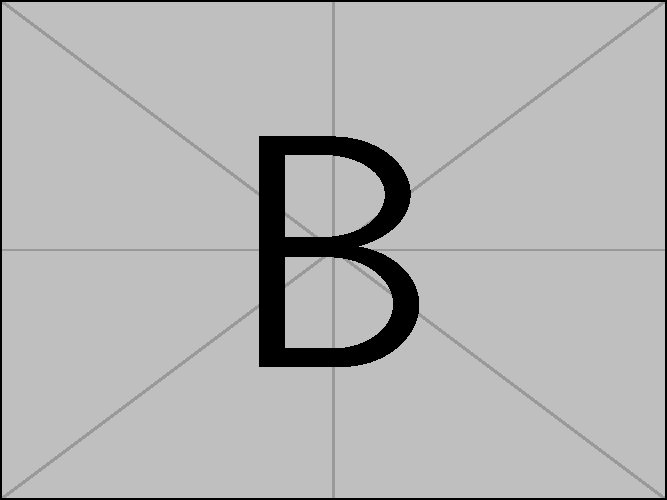
\includegraphics[width=0.45\linewidth]{example-image-b.pdf}}
  \caption{多个分图的示例}
  \label{fig:multi-image}
\end{figure}



\section{表格}

表应具有自明性。为使表格简洁易读，尽可能采用三线表，如表~\ref{tab:three-line}。
三条线可以使用 \pkg{booktabs} 宏包提供的命令生成。

\begin{table}[htbp]
  \centering
  \caption{三线表示例}
  \begin{tabular}{ll}
    \toprule
    文件名          & 描述                         \\
    \midrule
    bnuthesis.dtx   & 模板的源文件，包括文档和注释 \\
    bnuthesis.cls   & 模板文件                     \\
    bnuthesis-*.bst & BibTeX 参考文献表样式文件    \\
    bnuthesis-*.bbx & BibLaTeX 参考文献表样式文件  \\
    bnuthesis-*.cbx & BibLaTeX 引用样式文件        \\
    \bottomrule
  \end{tabular}
  \label{tab:three-line}
\end{table}

表格如果有附注，尤其是需要在表格中进行标注时，可以使用 \pkg{threeparttable} 宏包。
本例采用英文小写字母 a、b、c 等作为表内附注标记，与正文按页编号的脚注区分。

\begin{table}[htbp]
  \centering
  \begin{threeparttable}[c]
    \caption{带附注的表格示例}
    \label{tab:three-part-table}
    \begin{tabular}{ll}
      \toprule
      文件名                 & 描述                         \\
      \midrule
      bnuthesis.dtx\tnote{a} & 模板的源文件，包括文档和注释 \\
      bnuthesis.cls\tnote{b} & 模板文件                     \\
      bnuthesis-*.bst        & BibTeX 参考文献表样式文件    \\
      bnuthesis-*.bbx        & BibLaTeX 参考文献表样式文件  \\
      bnuthesis-*.cbx        & BibLaTeX 引用样式文件        \\
      \bottomrule
    \end{tabular}
    \begin{tablenotes}
      \item [a] 可以通过 xelatex 编译生成模板的使用说明文档；
        使用 xetex 编译 \file{bnuthesis.ins} 时则会从 \file{.dtx} 中去除掉文档和注释，得到精简的 \file{.cls} 文件。
      \item [b] 更新模板时，一定要记得编译生成 \file{.cls} 文件，否则编译论文时载入的依然是旧版的模板。
    \end{tablenotes}
  \end{threeparttable}
\end{table}

如某个表需要转页接排，可以使用 \pkg{longtable} 宏包，需要在随后的各页上重复表的编号。
编号后跟表题（可省略）和“（续）”，置于表上方。续表均应重复表头。
下表使用空白占位行演示跨页接排，不包含实验或调查数据。

% 先输出前面的浮动表格，避免后面的非浮动长表先于表 2 出现。
% \clearpage
\begin{longtable}{cccc}
    \caption{跨页长表格的表题} \\
    \toprule
    表头 1 & 表头 2 & 表头 3 & 表头 4 \\
    \midrule
  \endfirsthead
    \caption[]{跨页长表格的表题（续）} \\
    \toprule
    表头 1 & 表头 2 & 表头 3 & 表头 4 \\
    \midrule
  \endhead
    \bottomrule
  \endfoot
  Row 1  & & & \\
  Row 2  & & & \\
  Row 3  & & & \\
  Row 4  & & & \\
  Row 5  & & & \\
  Row 6  & & & \\
  Row 7  & & & \\
  Row 8  & & & \\
  Row 9  & & & \\
  Row 10 & & & \\
  Row 11 & & & \\
  Row 12 & & & \\
  Row 13 & & & \\
  Row 14 & & & \\
  Row 15 & & & \\
  Row 16 & & & \\
  Row 17 & & & \\
  Row 18 & & & \\
  Row 19 & & & \\
  Row 20 & & & \\
  Row 21 & & & \\
  Row 22 & & & \\
  Row 23 & & & \\
  Row 24 & & & \\
  Row 25 & & & \\
  Row 26 & & & \\
  Row 27 & & & \\
  Row 28 & & & \\
  Row 29 & & & \\
  Row 30 & & & \\
  Row 31 & & & \\
  Row 32 & & & \\
  Row 33 & & & \\
  Row 34 & & & \\
  Row 35 & & & \\
  Row 36 & & & \\
  Row 37 & & & \\
  Row 38 & & & \\
  Row 39 & & & \\
  Row 40 & & & \\
  Row 41 & & & \\
  Row 42 & & & \\
  Row 43 & & & \\
  Row 44 & & & \\
  Row 45 & & & \\
  Row 46 & & & \\
  Row 47 & & & \\
  Row 48 & & & \\
  Row 49 & & & \\
  Row 50 & & & \\
\end{longtable}

% !TeX root = ../bnuthesis-example.tex

\chapter{数学符号和公式}

\section{数学符号与计量单位}

数学符号应在全文中统一，首次出现时说明含义。本例在导言区保留了 \verb|math-style = TeX| 和 \verb|math-font = newcm| 的设置；作者应结合学科惯例统一选择符号样式，不宜在正文中反复切换。

常数和函数名可用正体表示，例如圆周率 $\uppi$、虚数单位 $\symup{i}$、函数 $\sin x$ 和自然对数 $\ln x$。微分符号使用本例定义的 \cs{dif} 命令，如 $\dif y/\dif x$；有限增量使用 $\increment x$。向量可以使用粗斜体，如 $\symbf{x}$。

计量单位可用 \pkg{siunitx} 宏包处理，以统一数值、单位和空白。例如：\SI{6.4e6}{m}、\SI{9}{\micro\meter}、\si{kg.m.s^{-1}} 和 \SIrange{10}{20}{\degreeCelsius}。这些数值只用于展示排版，不表示实验测量结果。

\section{单行与多行公式}

公式另起一行居中书写，序号置于所在行最右侧并加圆括号。引用公式时使用 \cs{eqref}，例如式~\eqref{eq:example}。式中 $x$ 为实数变量，积分上下限分别为零和圆周率。
\begin{equation}
  \int_0^{\uppi} \sin x\,\dif x = 2.
  \label{eq:example}
\end{equation}

多行公式应在运算或关系符号处换行，可使用 \env{align} 对齐。对于实数参数 $a$ 和 $b$，有
\begin{align}
  (a+b)^2
    &= a^2 + 2ab + b^2, \\
  (a-b)^2
    &= a^2 - 2ab + b^2.
\end{align}
复杂分式和多行公式应检查上下行间距，避免上下标、分式或积分限重叠。

\section{数学定理与证明}

定理环境可以使用 \pkg{amsthm} 或 \pkg{ntheorem} 宏包配置，本例保留 \pkg{amsthm}。下面的定理和证明用于演示环境的使用。

\begin{theorem}
  对任意实数 $a$ 和 $b$，均有
  \begin{equation}
    a^2+b^2 \ge 2ab.
    \label{eq:square-inequality}
  \end{equation}
  等号成立当且仅当 $a=b$。
\end{theorem}
\begin{proof}
  因为 $(a-b)^2\ge 0$，展开并移项得到式~\eqref{eq:square-inequality}。平方等于零当且仅当 $a-b=0$，故等号成立当且仅当 $a=b$。
\end{proof}

模板还提供 \env{assumption}、\env{definition}、\env{proposition}、%
\env{lemma}、\env{theorem}、\env{axiom}、\env{corollary}、\env{exercise}、
\env{example}、\env{remar}、\env{problem}、\env{conjecture} 等环境。实际写作中，定理的前提、结论及证明应完整，并明确说明所引用的已有结果。

% !TeX root = ../bnuthesis-example.tex

\chapter{文献引用}

\section{引文与参考文献的一致性}

2026 年编写规则要求引文标注与参考文献表采用 GB/T 7714-2015，在顺序编码制或著者--出版年制中选择一种，并保持全文一致。全部被引文献都应进入参考文献表，未引用的文献不应混入其中。

本例按已确认的例外，保留 \file{bnuthesis-author-year-bnu.bst} 对文献表的著者排序，并用数字上标标注正文引用。这一组合需要培养单位认可，不能作为规则规定的标准配套方式。中文文献的著者排序依赖数据库中的拼音 \texttt{key} 字段，新增条目时须补充并核对该字段。

\section{本例使用的引用方式}

本例使用 BibTeX 与 \pkg{natbib}，全文保持相同的数字上标格式。例如，期刊论文\cite{zhangkun1994}、专著\cite{zhukezhen1973} 和学位论文\cite{zhengkaiqing1987} 可以分别引用。同一位置引用多篇文献时，将键写在同一命令内\cite{zhangkun1994,zhukezhen1973}。

下面给出命令和排版结果的对应关系，各行均使用当前引用制度。
\begin{center}
  \begin{tabular}{ll}
    \toprule
    命令 & 结果 \\
    \midrule
    \verb|\cite{zhangkun1994}| & \cite{zhangkun1994} \\
    \verb|\citet{zhangkun1994}|              & \citet{zhangkun1994}              \\
    \verb|\citep{zhangkun1994}|              & \citep{zhangkun1994}              \\
    \verb|\cite[42]{zhukezhen1973}| & \cite[42]{zhukezhen1973} \\
    \verb|\cite{zhangkun1994,zhukezhen1973}| & \cite{zhangkun1994,zhukezhen1973} \\
    \bottomrule
  \end{tabular}
\end{center}

数据库中还保留了原有的其他文献条目，只有在正文中被引用的条目才输出到文献表。概率论专著\cite{peebles2001probability} 在此作为外文专著的著录示例，不表示本例进行了相应的研究。

\section{其他配套方式的代码说明}

若采用标准顺序编码制，可在导言区选用数字文献表样式，按引用顺序著录。以下仅展示代码，不在本例正文中执行：
\begin{verbatim}
\usepackage[sort]{natbib}
\bibliographystyle{bnuthesis-numeric}
\end{verbatim}

若采用标准著者--出版年制，应同时更换文献表样式和正文标注方式，并将中文文献按著者字顺和年份排列。以下也仅作代码说明：
\begin{verbatim}
\usepackage{natbib}
\bibliographystyle{bnuthesis-author-year}
\bnusetup{cite-style = author-year}
\end{verbatim}

修改参考文献方案后，应完整运行 LaTeX、BibTeX 和后续 LaTeX 编译，检查是否有未解析的引用以及正文与文献表不对应的条目。

\cite{zhangkun1994,zhukezhen1973,dupont1974bone,zhengkaiqing1987,%
  jiangxizhou1980,jianduju1994,merkt1995rotational,mellinger1996laser,%
  bixon1996dynamics,mahui1995,carlson1981two,taylor1983scanning,%
  taylor1981study,shimizu1983laser,atkinson1982experimental,%
  kusch1975perturbations,guangxi1993,huosini1989guwu,wangfuzhi1865songlun}

\cite{zhaoyaodong1998xinshidai,biaozhunhua2002tushu,chubanzhuanye2004,%
  who1970factors,peebles2001probability,baishunong1998zhiwu,%
  weinstein1974pathogenic,hanjiren1985lun,dizhi1936dizhi,%
  tushuguan1957tushuguanxue,aaas1883science,fugang2000fengsha,%
  xiaoyu2001chubanye,oclc2000about,scitor2000project%
}

% !TeX root = ../bnuthesis-example.tex

\chapter{结论}

本示例展示了中文学术博士学位论文的组成、页面样式和常用排版元素，说明了图表、公式、定理及文献引用的基本用法，并通过两份附录演示独立编号。所有示意内容均服务于模板使用，不代表作者取得了相应科研成果。

实际论文的结论应概括主要研究结果及其意义，明确创新点、适用范围和局限，并在需要时提出后续研究方向。结论应与正文中的证据相互对应，避免将章节提纲或各章小结简单拼接，也不应在缺少证据时使用“首次”“领先”等判断。

提交前应以正式材料替换学术成果和答辩委员会名单的占位内容，核对中英文摘要、图表及公式编号、引文与参考文献、页眉页码及打印封皮，并结合培养单位的补充要求逐项检查。



% 其他部分
\backmatter

% 参考文献
\bibliography{ref/refs}  % 参考文献使用 BibTeX 编译
% \printbibliography       % 参考文献使用 BibLaTeX 编译

% 附录
\appendix
% !TeX root = ../bnuthesis-example.tex

\chapter{图表和公式的补充示例}

附录是与论文内容密切相关、但编入正文又影响整篇论文编排的条理和逻辑性的资料，例如某些重要的数据表格、计算程序、统计表等，是论文主体的补充内容，可根据需要设置。
本例设置两份附录，展示图、表、公式如何随附录重新编号，正文页码保持连续。


\section{图表示例}

\subsection{图}

附录中的图片示例（图~\ref{fig:appendix-figure}）。

\begin{figure}[htbp]
  \centering
  
\includegraphics[width=0.6\linewidth]{example-image-a.pdf}
  \caption{附录中的图片示例}
  \label{fig:appendix-figure}
\end{figure}


\subsection{表格}

附录中的表格示例（表~\ref{tab:appendix-table}）。

\begin{table}[htbp]
  \centering
  \caption{附录中的表格示例}
  \begin{tabular}{ll}
    \toprule
    文件名          & 描述                         \\
    \midrule
    bnuthesis.dtx   & 模板的源文件，包括文档和注释 \\
    bnuthesis.cls   & 模板文件                     \\
    bnuthesis-*.bst & BibTeX 参考文献表样式文件    \\
    bnuthesis-*.bbx & BibLaTeX 参考文献表样式文件  \\
    bnuthesis-*.cbx & BibLaTeX 引用样式文件        \\
    \bottomrule
  \end{tabular}
  \label{tab:appendix-table}
\end{table}


\section{数学公式}

附录中的数学公式示例（公式~\eqref{eq:appendix-equation}）。
\begin{equation}
  \int_a^b f(x)\,\dif x = -\int_b^a f(x)\,\dif x.
  \label{eq:appendix-equation}
\end{equation}
其中，$f$ 是在端点 $a$ 和 $b$ 之间可积的函数。

\chapter{第二份附录的独立编号}

第二份附录用于核对图~\ref{fig:appendix-b-figure}、表~\ref{tab:appendix-b-table} 和式~\eqref{eq:appendix-b-equation} 的序号是否从 B1 开始，避免沿用第一份附录或正文的编号。

\begin{figure}[htbp]
  \centering
  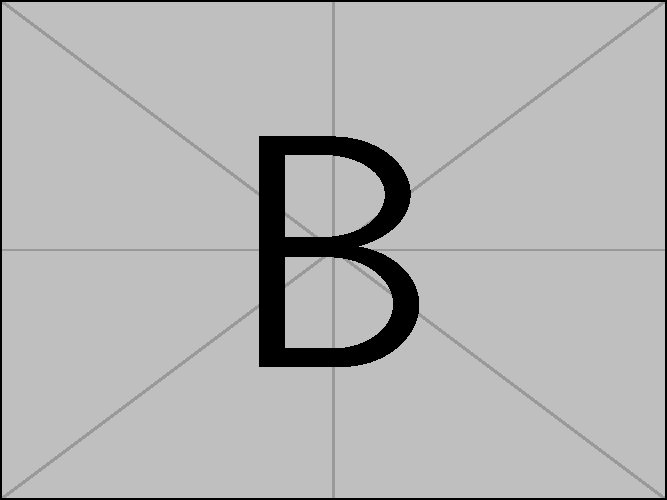
\includegraphics[width=0.6\linewidth]{example-image-b.pdf}
  \caption{第二份附录的图片示例}
  \label{fig:appendix-b-figure}
\end{figure}

\begin{table}[htbp]
  \centering
  \caption{附录编号检查项目}
  \label{tab:appendix-b-table}
  \begin{tabular}{ll}
    \toprule
    项目 & 检查内容 \\
    \midrule
    图与表 & 各附录分别从 1 开始 \\
    公式 & 使用所属附录字母与序号 \\
    页码 & 与正文及其他文后部分连续 \\
    \bottomrule
  \end{tabular}
\end{table}

对正整数 $n$，以 $k$ 为求和指标，有
\begin{equation}
  \sum_{k=1}^{n} k = \frac{n(n+1)}{2}.
  \label{eq:appendix-b-equation}
\end{equation}


% 索引为可选部分。本例演示主题条目与页码引用，不需要时注释下一行。
% !TeX root = ../bnuthesis-example.tex

% 索引为可选部分，放在附录之后、成果列表之前。
% 不使用 \chapter{索引}，避免被编为“附录 C”。
\chapter*{\indexname}
\phantomsection
\addcontentsline{toc}{chapter}{\indexname}
\markboth{\indexname}{\indexname}

\begingroup
  \normalfont\songti\fontsize{12bp}{20bp}\selectfont
  \setlength{\parindent}{2\ccwd}
  \setlength{\parskip}{0bp}

  本索引按汉语拼音字顺编排，示例收录正文和附录中的部分主题、概念与术语。
  条目后的数字为相关内容所在页码；“见”表示同义词参照。

  % 字母分组是本例采用的检索方式，并非学校要求的固定版式。
  % 按实际论文内容增删条目并人工核对拼音排序，尤其注意多音字。
  % 页码引用正文中已有的标签；新增条目时，在对应内容处设置 \label。
  % 多个页码按升序列出，同页只保留一次；连续页可写 \pageref{起点}--\pageref{终点}。
  \textbf{B}\par\nopagebreak[4]
  表格，\pageref{tab:three-line}\par

  \textbf{C}\par\nopagebreak[4]
  插图，\pageref{fig:example}，\pageref{fig:multi-image}\par

  \textbf{D}\par\nopagebreak[4]
  带附注的表格，\pageref{tab:three-part-table}\par
  定理，\pageref{eq:square-inequality}\par

  \textbf{F}\par\nopagebreak[4]
  分图，\pageref{fig:multi-image}\par
  附录，\pageref{fig:appendix-figure}，\pageref{fig:appendix-b-figure}\par

  \textbf{G}\par\nopagebreak[4]
  公式，\pageref{eq:example}，\pageref{eq:appendix-equation}，\pageref{eq:appendix-b-equation}\par

  \textbf{J}\par\nopagebreak[4]
  积分，\pageref{eq:example}，\pageref{eq:appendix-equation}\par

  \textbf{S}\par\nopagebreak[4]
  三线表，\pageref{tab:three-line}\par

  \textbf{T}\par\nopagebreak[4]
  图片，见“插图”\par
\endgroup


% 攻读学位期间取得的学位论文相关成果
% !TeX root = ../bnuthesis-example.tex

\begin{resume}
  以下为待填写项目，不表示作者已经发表论文、取得专利或完成其他科研成果。提交前应根据真实记录列出攻读学位期间发表或已录用的论文及其他与学位论文相关的成果；没有相应成果时，应按培养单位要求说明。

  \section*{学术论文}
  \begin{achievements}
    \item 待填写：作者．论文题名［文献类型］．期刊名称，年份，卷（期）：页码．本人作者排名与署名单位：待填写；发表或录用状态及年月：待填写。
  \end{achievements}

  \section*{软件著作}
  \begin{achievements}
    \item 待填写：成果名称、成果类型、完成人及本人排名、完成或授权年月、署名单位和必要的证明信息。
  \end{achievements}

  \section*{参与项目}
  \begin{achievements}
    \item 待填写：成果名称、成果类型、完成人及本人排名、完成或授权年月、署名单位和必要的证明信息。
  \end{achievements}

\end{resume}


% 致谢
% !TeX root = ../bnuthesis-example.tex

\begin{acknowledgements}
  本页为致谢内容的占位说明，提交前应由作者根据实际情况重写。致谢可以向提供资助、指导和协助完成论文研究的单位及个人表示感谢，叙述应实事求是、真诚客观。

  如需列出资助项目，应核对项目名称、编号及致谢要求；如需提及合作研究、访问经历或他人的具体贡献，应以真实经历及实际工作为依据。本例不预设作者获得的资助或已有的合作经历。
\end{acknowledgements}


% 答辩委员会名单位于致谢之后，使用正式名单替换占位信息。
% !TeX root = ../bnuthesis-example.tex

\begin{committee}[name={答辩委员会名单}]
  \begin{center}
    \begin{tabular}{@{}p{1.5cm}p{1.6cm}p{4.3cm}p{1.8cm}p{2.8cm}@{}}
      \toprule
      职务 & 姓名   & 工作单位 & 职称   & 导师类型 \\
      \midrule
      主席 & 待填写 & 待填写   & 待填写 & 待填写   \\
      委员 & 待填写 & 待填写   & 待填写 & 待填写   \\
      委员 & 待填写 & 待填写   & 待填写 & 待填写   \\
      委员 & 待填写 & 待填写   & 待填写 & 待填写   \\
      委员 & 待填写 & 待填写   & 待填写 & 待填写   \\
      \bottomrule
    \end{tabular}
  \end{center}
\end{committee}


\end{document}
